\documentclass{article}
\usepackage{graphicx}


\begin{document}

    \title{Freelancing Management System \\
    \textbf{FMS}}
    \author{\textit{The Team --- Yaser, Umar, Taha and Boda}}
    \date{March 25, 2017}
\maketitle

\begin{figure}[ht!]
\centering
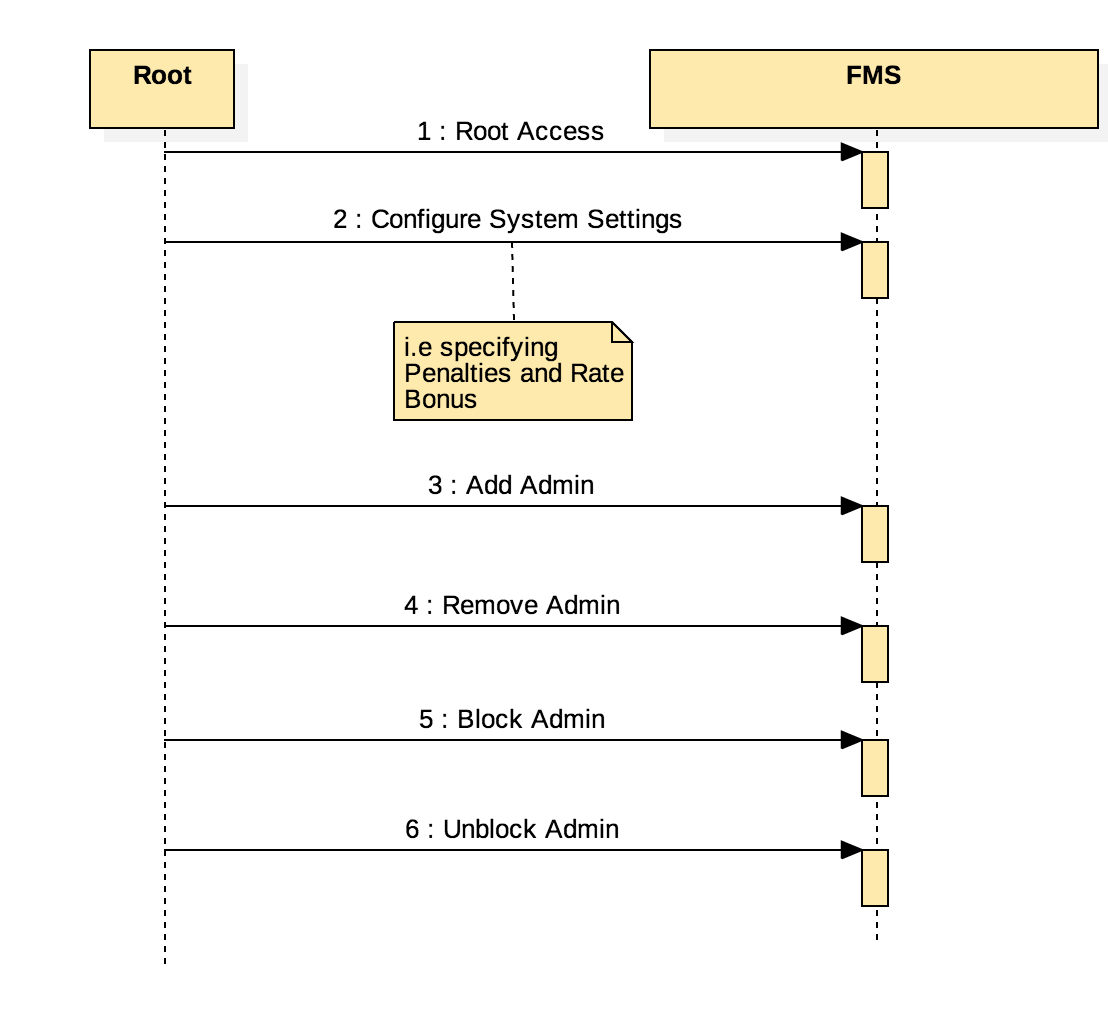
\includegraphics[width=128mm]{SystemSequanceDiagram_Root.png}
\caption{System Sequance Diagram of the \textit{Root}}
\end{figure}

\newpage
\tableofcontents
\newpage



\section{System Description}
  \hspace{0.5cm} This is a \textit{Freelancing Management System}, a system which
  allows \textit{Customers } and \textit{Freelancers} to find
  one--another easily. It manages the processes from finding workers,
  verifying them, engaging, paying up to rating.
  \hspace{0.3cm}Let us take you on an interesting tour into the
  \textit{system actors}, every one of them sees the system differently
  according to their role.

\subsection{Root}
\hspace{0.5cm} \textit{The Root} is the owner of the system. He is the one
who set it up for the first time with a special root access from him.


\subsection{Admin}
\subsection{Freelancer}
\subsection{Employer}




\section {Diagrams}
These diagrams abstract FMS due to several points of views
\subsection{Domain Diagram}
\subsection{Class Diagram}
\subsection{Use Case Diagram}
\subsection{Class Diagram}
\subsection{System Sequance Diagrams}

\section{Call Us}





\end{document}
